\documentclass{standalone}

\usepackage{tikz}
\usepackage{amsmath}
\usepackage{unicode-math}
\usepackage{xcolor}
\colorlet{darkRed}{red!40!black}
\colorlet{darkBlue}{cyan!50!black}
\colorlet{darkYellow}{yellow!50!black}


\begin{document}

\usetikzlibrary{calc}

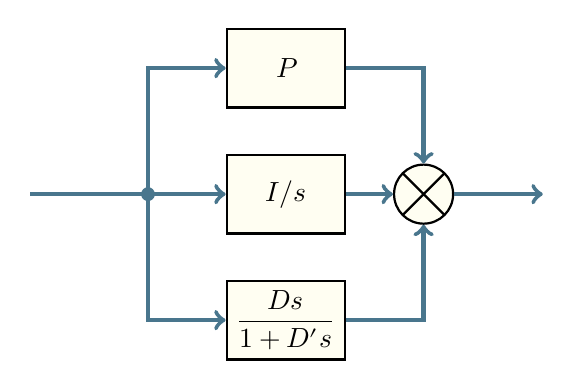
\begin{tikzpicture}[
    thick,
    arr/.style={ultra thick, draw=darkBlue},
    err/.style={ultra thick, draw=darkRed},
    box/.style={
        rectangle,
        minimum width=1.5cm,
        minimum  height=1cm,
        draw=black,
        align=center,
        fill=yellow!5,
      },
    cross/.style={path picture={
            \draw[black]
            (path picture bounding box.south east) -- (path picture bounding box.north west) (path picture bounding
            box.south west)
            -- (path picture bounding box.north east);
          }},
    sum/.style={circle, minimum size=.75cm, draw=black, cross, fill=yellow!5},
    ma/.style={midway, above},
    mb/.style={midway, below},
    ml/.style={midway, left},
  ]
  \node[box] (P) at (2.5,+1.6) {$P$};
  \node[box] (I) at (2.5,+0) {$I / s$};
  \node[box] (D) at (2.5,-1.6) {$\dfrac{Ds}{1 + D's}$};
  \node[sum] (sum) at (4.25,0) {};

  \node[circle, minimum size=5pt, fill=darkBlue, inner sep=0] (T) at (.75,0) {};

  \draw[arr, -to] (T.center) |- (P);
  \draw[arr, -to] (T.center) -- (I);
  \draw[arr, -to] (T.center) |- (D);

  \draw[arr, -to] (P) -| (sum.90);
  \draw[arr, -to] (I) -- (sum.180);
  \draw[arr, -to] (D) -| (sum.270);

  \draw[arr] (T.center) -- ++(-1.5,0);
  \draw[arr, -to] (sum.0) -- ++(1.125,0);
\end{tikzpicture}
\end{document}
